\newpage
\refstepcounter{section}
%Add Image
\vspace*{-40mm} %Make image have no top margin
\begin{tikzpicture}
\node[inner sep=0pt] (x) at (0,0)
    {\hspace{-87mm}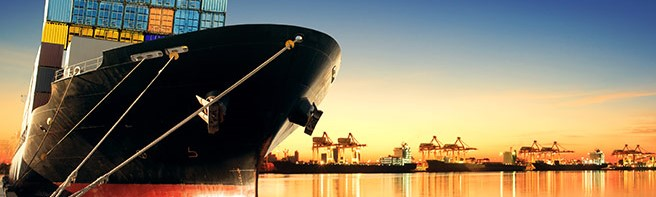
\includegraphics[width=\paperwidth]{sectionimage1.jpg}};
\node[text width=10in] (Z) at (0,-1) {\color{white}\headingfont\Large\bfseries\uppercase{\hspace{-0.7cm}\thesection\hspace{0.5cm}Best Fit Option}};
\end{tikzpicture}
%Modify TOC
\addcontentsline{toc}{section}{\protect\numberline{\thesection}Best Fit Option}
  \sectionmark{Best Fit Option}

\subsection*{Initial Best-fit Solution}
Following extensive research into possible Port relocation options, a M.A.R.T analysis was conducted to determine the viability of each option with consideration of the stakeholder requirements. This looked to analyse economic, environmental and societal aspects as well as the overall feasibility of the option. Each of these aspects were considered in terms of the key stakeholder requirements and weighted according to importance to help determine the best fit solution. Any underdeveloped areas were further iterated to establish a final solution that best fit the requirements and aims of the project. 
\\Out of the four considered options, keeping the Port of Auckland as is and the relocation of the Port of Auckland to Tauranga were determined to be the top two solutions closest to meeting the decided requirements. From the M.A.R.T analysis, it was clear relocating to Tauranga was the best fit option, this is especially prevalent when considering the points below:
\begin{itemize}[noitemsep]
    \vspace{-2mm}
    \item PoA would eventually need to expand and anticipate the need for change to allow for a smooth transition to better meet the public's approval (people want the waterfront area used for purposes other than freight).
    \item Redistributions of population densities and development of different regional areas
    \item Reduction of traffic congestion in Auckland.
    \item Tauranga is not at capacity yet and has potential to grow.
\end{itemize}
\subsection*{Justification}
Keeping the PoA in Auckland would see it heavily restricted in its future developments and it cannot solely maintain the predicted freight capacity that New Zealand hopes to support. Current congestion in the CBD reduces efficiency significantly and delaying the redistributions of freight traffic will come at a higher capital cost in the long term. 
\\The sole movement of freight traffic to Whangarei is not supported by a reliable transport network. The NAL is showing significant signs of wear and does not have the capacity to move the required volume of freight from Whangarei to Auckland. The costs of refurbishing and expanding the line would not justify the economic benefit of moving the PoA to Northland. 
\\Relocating the port hubs to both Port of Tauranga and Northport would require the upgrade of transport networks in both northbound and southbound directions to Whangarei and Tauranga respectively inducing heavy and unrealistic capital costs outweighing any social and economic benefits provided by the distribution of wealth.
\\In the first analysis, a relocation of the Port of Auckland to Tauranga proved to satisfy most of the Stakeholder Requirements. It reduced traffic congestion within Auckland and allowed for freight to be distributed efficiently around the North Island as Tauranga is located within the ‘Golden Triangle’. This proved to be more economically feasible in comparison to relocating the Port to Whangarei or a combination and also provided the best economic value and growth for the North Island. However, when the option was compared to the original Stakeholder Requirements, the complete relocation of the Port to Tauranga contained risks and options needed to be recycled to iterate for a better solution.
\subsection*{Optioneering}
Despite the Port of Tauranga being considered as the ‘least-worst’ of the four initial option, when compared to the project and stakeholder requirements, it was identified that the PoT alone would not have sufficient capacity to accommodate for Auckland’s freight traffic alongside its own. Additionally, the current transport infrastructure between Hamilton and Tauranga does not allow for redundancy in the event of damage.
\subsection*{Development of a Secondary Port around the Auckland Region}
\subsubsection*{Relocate the Port to Kawakawa Bay}
While Kawakawa Bay has sufficient draught capacity, a relocation of the Port would require the construction of significant infrastructure to make freight transport feasible. The lack of major transport infrastructure would exert exorbitant capital costs on the project. The location of the port also raises important cultural, social and environmental issues.
\subsubsection*{Relocate Port to Manukau}
Manukau Harbour is located on the west side of New Zealand, away from current shipping routes, which may result in increased shipping costs and a decrease in efficiency. Manukau’s high population density also limits port expansion. The shifting sandbar makes entrance into the Harbour difficult and would require constant dredging. Because it is located on Maori land, legislations and consents would be required for the project to proceed. 
\subsection*{Best Fit Option}
Given this analysis, retaining approximately 20\% of the existing PoA is the most feasible option as it allows for gradual relocation and builds redundancy into the design. Given that a split distribution between the Auckland and Tauranga Ports is the best option, freight transport infrastructure needs to be considered.
\subsection*{Development of Rail Lines}
Links between Auckland, Hamilton and Tauranga, need to be developed to the standard that would be required to handle the predicted freight transport capacity. Enhancing the current rail is part of the Regional Rapid Rail (RRR) passenger and freight transport plan developed by Labour Government. Any new freight lines developed for the PoT would follow the construction schedule of the RRR plan to streamline fabrication. The upgrade of the East Coast Main Trunk to a double rail line would increase the rail freight capacity. Another benefit of having two rails is that the other serves as a safeguard from accidents such as slips which threaten rail closures. 
\subsection*{Development of Road}
The sheer volume of freight requires multiple modes of transport. Upgrading the two-lane-two-way road over the Kaimai Ranges to a four-lane-two-way road will provide an alternative freight route to the existing rail line. In the case of natural disasters such as earthquakes or landslides, roads can also be utilised as a viable alternative to rail.
\\\newline This recycling process was beneficial as it allowed for ‘stakeholder feedback’, and with each iteration, modifications were made that improved the solution’s overall functional capability and better satisfied the problem.



\subsection*{Revised Best Fit Solution}

After analysing previous options, and referring back to our stakeholder requirements, it was determined that the option of moving all of PoA’s freight traffic to PoT was not technically feasible or efficient in the long term. It was then decided over an iterative process that the best solution was to minimise the port of Auckland to 20\% over a period of 10 years and transfer the excess shipping traffic to the PoT. This best fit option includes the gradual expansion of the PoT to compensate for the increase in freight traffic and the upgrade of the East Coast Main Trunk between the Hamilton and Tauranga ports. The connecting state highways will also be upgraded to further aid in freight transport as well as covering the risk of natural disasters such as landslides, and their effect in blocking trade routes.

\begin{figure}
\centering
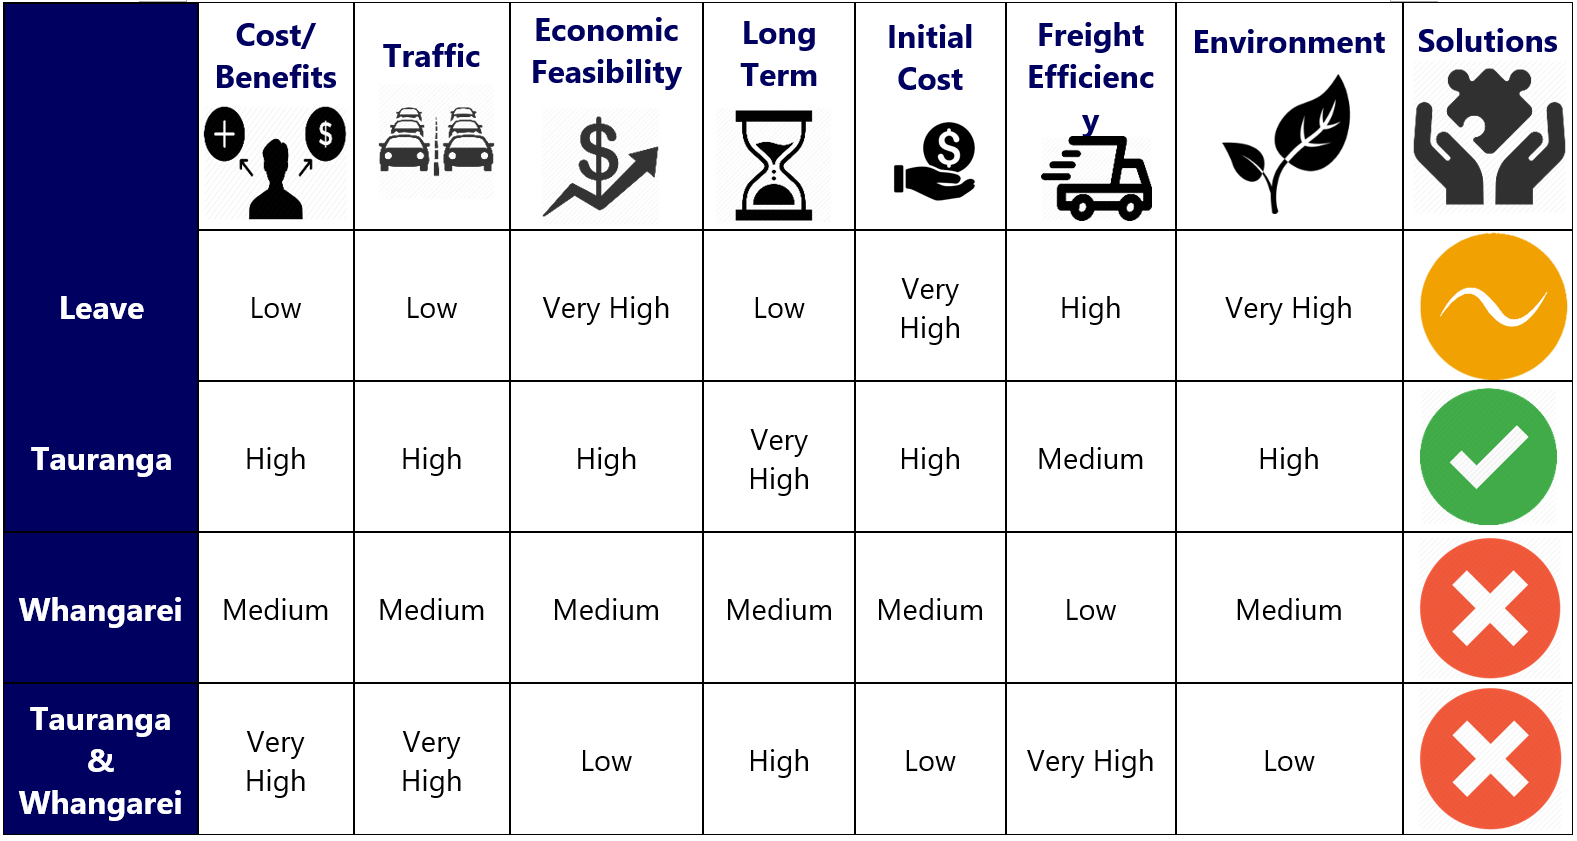
\includegraphics[width=0.9\textwidth]{mart1.png}
\centering
\caption{MART Analysis}
\end{figure}
\begin{figure}
\centering
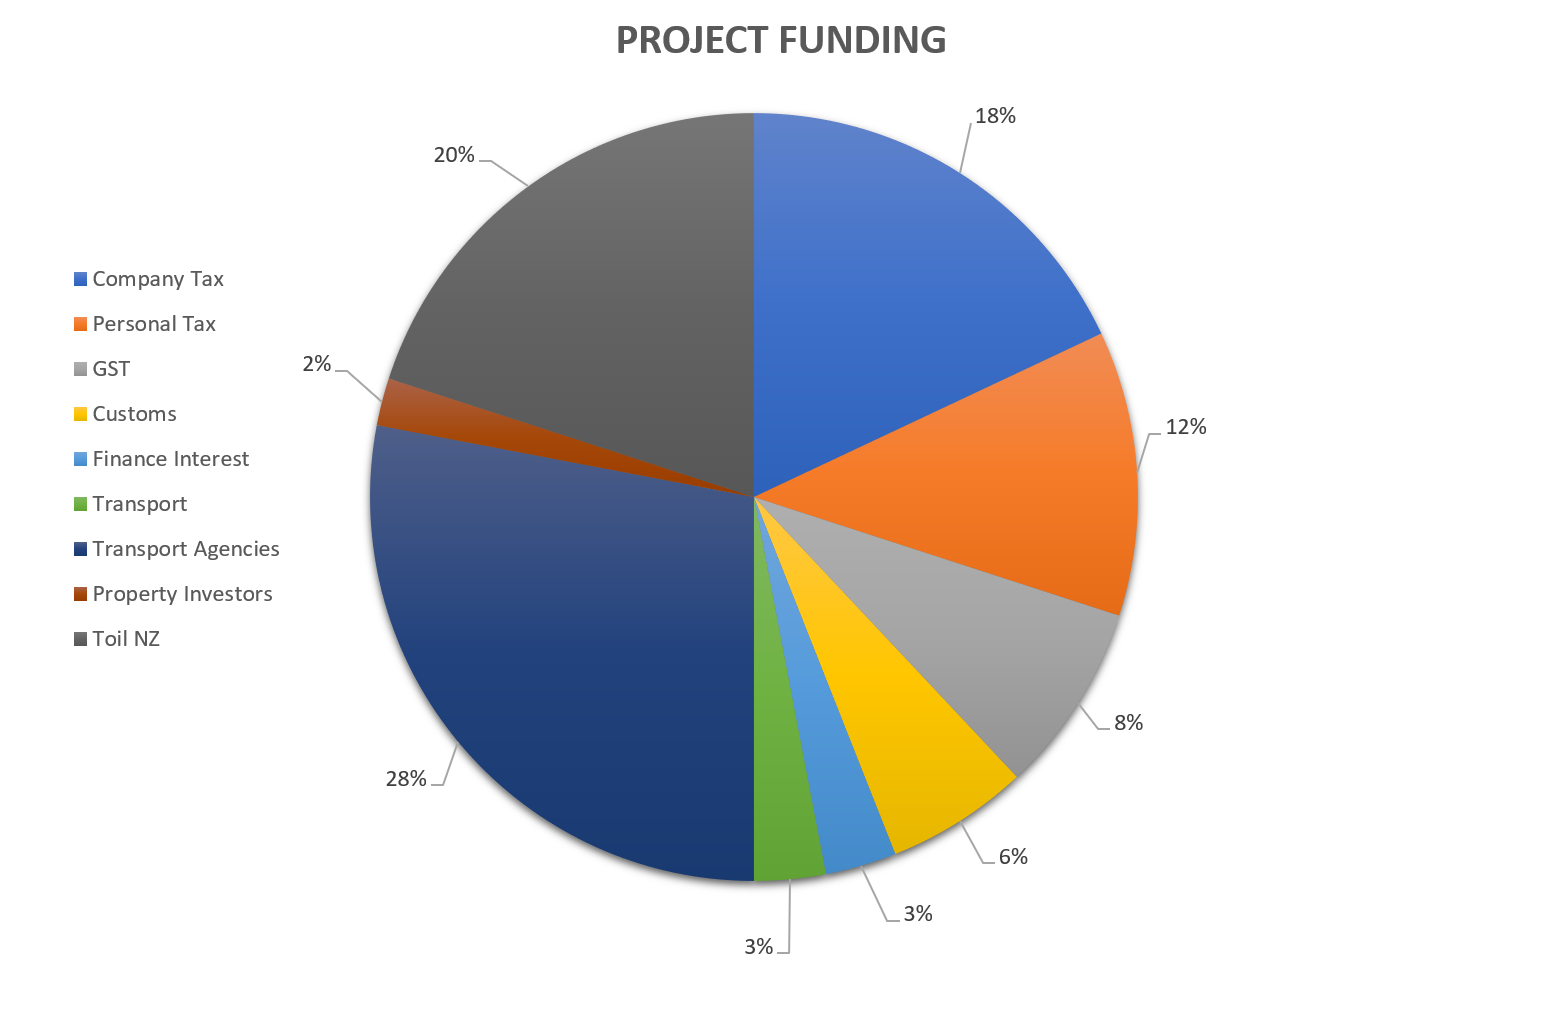
\includegraphics[width=0.7\textwidth]{ProjectFunding.png}
\centering
\caption{Project Funding}
\end{figure}


\clearpage